\chapter{实战练习}
\begin{tikzpicture}[smooth]
\draw[arrows={-Stealth[length=5pt, inset=3.5pt]}] (-0.5,0) -- (3.0,0)node (xaxis) [right=-1pt] {$x$};
\draw[arrows={-Stealth[length=5pt, inset=3.5pt]}] (0,-0.5) -- (0,4.5)node (yaxis) [above=-0.6pt] {$y$};
\draw  (-0.18,-0.18) node {$o$};
\draw[color=red,domain=0:2.0,fill=green!20] plot (\x,4*\x-\x*\x);
\draw[color=red!40,domain=0:2.90] plot (\x,4*\x-\x*\x)  ;
\draw[color=blue!30,domain=0:2.3] plot (\x,2*\x)  ;
\draw[fill=black] (2,4) circle [radius=0.2pt] node[above=-1.8pt] {$\scaleobj{0.8}{A(2,4)}$};
\end{tikzpicture}   
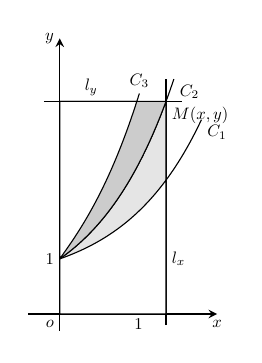
\begin{tikzpicture}[yscale=0.7]
\draw[-stealth] (-0.4,0)--(2,0) node[below,scale=0.6]{$x$};
\draw[-stealth] (0,-0.3)--(0,5) node[left,scale=0.6]{$y$};
\draw (0,0) node [below left,scale=0.6] {$o$};
\foreach \i in {1}{\draw (\i,0)--node [below,scale=0.6] {$1$}(\i,0.05);}
\draw (0,1) node [left,scale=0.6] {$1$};
\draw (1.35,1) node [right,scale=0.6] {$l_x$};
\draw (0.4,3.85742) node [above,scale=0.6] {$l_y$};
\draw (1.35,-0.2) -- (1.35,4.25519);
\draw (-0.2,3.85742) -- (1.55,3.85742);
\draw (1.35,3.85742) node [below right,scale=0.6] {$M(x,y)$};
%\clip (-1,-1) rectangle (5,5);%只在这个区域内画图
\draw[domain=1:4,smooth,variable=\t] plot ({ln(\t)+1/(2*\t)-0.5},\t)node[above,scale=0.6] {$C_3$};
\draw[domain=0:1.8,smooth] plot (\x,{0.5*1+0.5*exp(\x)}) node[below right,scale=0.6] {$C_1$};
\draw[domain=0:1.45,smooth] plot (\x,{exp(\x)}) node[below right,scale=0.6] {$C_2$};
\filldraw [fill=gray!20] (0,0) -- plot [domain=0:1.35,smooth] (\x,{exp(\x)}) -- (1.35,0) -- (0,0);
\filldraw [fill=white] (0,0) -- plot [domain=0:1.35,smooth] (\x,{0.5*1+0.5*exp(\x)}) -- (1.35,0) -- (0,0);
\filldraw [fill=gray!40] (0,1) -- plot [domain=0:1.35,smooth] (\x,{exp(\x)}) -- (0,3.85742) -- (0,1);
\filldraw [fill=white] (0,1) -- plot [domain=1:3.85742,smooth,variable=\t] ({ln(\t)+1/(2*\t)-0.5},\t) -- (0,3.85742) -- (0,1);
\end{tikzpicture}

\begin{tikzpicture}[scale=1.5]
\draw[-stealth] (-0.3,0) -- (2.2,0)node (xaxis) [right,scale=0.8] {$x$};
\draw[-stealth] (0,-1.6) -- (0,1.6)node (yaxis) [left,scale=0.8] {$y$};
\fill[pink!] (0,0) -- (1,-1) arc [start angle=315, end angle=405, radius=1.414] -- (0,0);
\fill[pink!] (1,0) -- (1,1) arc [start angle=90, end angle=180, radius=1] -- (0,0);
\fill[grassgreen] (0,0) -- (1,-1) arc [start angle=315, end angle=360, radius=1.414] -- (1.414,0)--(2,0) arc [start angle=360, end angle=270, radius=1] -- (1,-1);
\fill[grassgreen] (0,0) -- (1,1) arc [start angle=45, end angle=0, radius=1.414] -- (1.414,0)--(2,0) arc [start angle=0, end angle=90, radius=1] -- (1,1);
\draw (1,-0.02)--(1,0.02) node[below] {$\scaleobj{0.6}{1}$};
\draw (1.414,-0.02)--(1.414,0.02) node[below] {$\scaleobj{0.6}{\sqrt{2}}$};
\draw[style=dashed,color=red,domain=-0.1:1.4] plot(\x,-\x);
\draw[color=black,domain=-0.1:2.2] plot(\x,0);
\draw[style=dashed] (0,0)--(0,-1.414) arc [start angle=270, end angle=450, radius=1.414];
\draw (1,0) circle [radius=1];
%\fill[pattern=north west lines](0,0)--(-2,0)--(-2,2)--(0,2)arc(90:270:0.8); 
%\fill[pattern=north west lines]arc(-45:0:1); 
\end{tikzpicture}
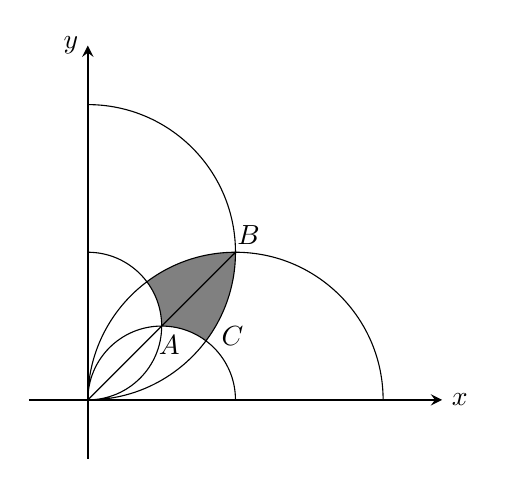
\begin{tikzpicture}[scale=15]
\begin{scope}
\clip (0,0) arc (-90:0:1/8) arc (90:180:1/8);
\fill[gray,even odd rule] (0,0) arc (-90:0:1/8) arc (90:180:1/8) 
arc (-90:270:1/16) arc (-180:180:1/16) arc (-90:0:1/16) arc (90:180:1/16);
\end{scope}
\draw [-stealth,thick](-0.05,0)--(0.3,0);
\draw [-stealth,thick](0,-0.05)--(0,0.3);
\node[right]at(0.3,0){$x$};
\node[left]at(0,0.3){$y$};
\draw (0,0) arc (-90:90:1/8) (0,0) arc (-90:90:1/16)
(0,0) arc (180:0:1/8) (0,0) arc (180:0:1/16) (0,0)--(1/8,1/8);
\node [below]at(0.069,0.0627){$A$};
\node [above]at(0.136,0.123){$B$};
\node [right]at(0.105,0.0541){$C$};
\end{tikzpicture}

\begin{tikzpicture}[scale=15]
\begin{scope}
\clip (0,0) arc (-90:0:1/8) arc (90:180:1/8);
\fill[pattern=horizontal lines]
(0,0) arc (-90:0:1/8) --(1/16,1/16) arc (90:0:1/16);
\fill[pattern=vertical lines]
(0,0) arc (180:90:1/8) --(1/16,1/16) arc (0:90:1/16);
\end{scope}
\draw [-stealth,thick](-0.05,0)--(0.3,0);
\draw [-stealth,thick](0,-0.05)--(0,0.3);
\node[right]at(0.3,0){$x$};
\node[left]at(0,0.3){$y$};
\draw (0,0) arc (-90:90:1/8) (0,0) arc (-90:90:1/16)
(0,0) arc (180:0:1/8) (0,0) arc (180:0:1/16) (0,0)--(1/8,1/8);
\node [below]at(0.069,0.0627){$A$};
\node [above]at(0.136,0.123){$B$};
\node [right]at(0.105,0.0541){$C$};
\end{tikzpicture}
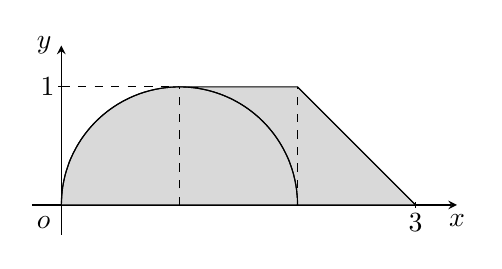
\begin{tikzpicture}[scale=1.5]
\begin{scope}
\draw[-stealth] (-0.25,0) -- (3.35,0) node (xaxis) [below] {$x$};
\draw[-stealth] (0,-0.25) -- (0,1.35) node (yaxis) [left] {$y$};
\draw (3,0.025)--(3,-0.025) node[below=-0.5mm] {3};
\draw (0.025,1) -- (-0.025,1) node[left=-0.75mm] {1};
\end{scope}
\draw  (-0.15,-0.15) node {$o$};
\draw[fill=gray!30] (2,0) arc [start angle=0, end angle=180, radius=1] -- (3,0) -- (2,1) -- (1,1); %,pattern=dots,even odd rule
\draw[domain=2:3,fill=green!20] plot (\x,3-\x);
\draw[samples=300,domain=0:2.0] plot (\x,{(1-(1-\x)^2)^(1/2)});
\draw[dashed] (0,1) -- (1,1);
\draw[dashed] (2,0) -- (2,1);
\draw[dashed] (1,0) -- (1,1);
\end{tikzpicture}	

\begin{tikzpicture}
\node[above,xscale=1.2,yscale=1.4]{\Huge\bfseries 欢迎同学们进行错误指正!};
\node[xscale=1.2,above,yscale=-1.4,scope fading=south,opacity=0.2]{\Huge\bfseries 欢迎同学们进行错误指正!};
\end{tikzpicture} 

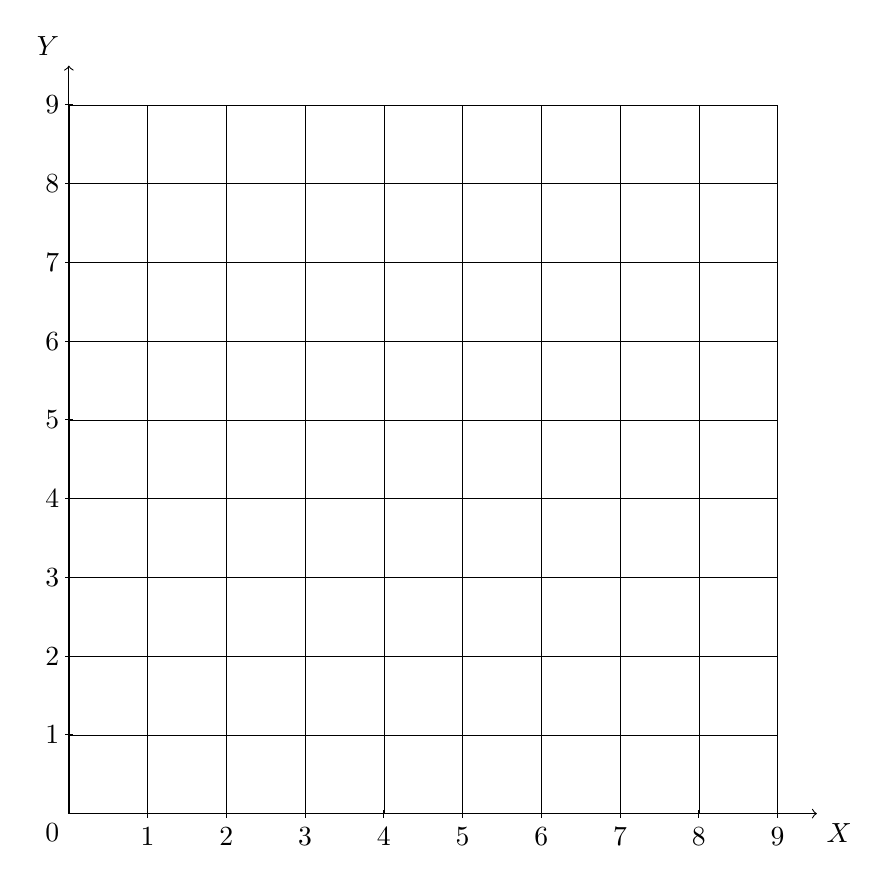
\begin{tikzpicture}
\draw[help lines,black] (0,0) grid (9,9); %网格线
\draw [->] (0,0)--(9.5,0) node[below right] { $X$};
\draw [->] (0,0)--(0,9.5) node[above left] {$Y$};
\node[below left] at (0,0) {0};
\foreach \i in {1,...,9}
\draw (\i,-0.05)--++(90:0.1) node[below=1mm]{\i};
%\draw (\i,-0.05)--(\i,0.05) node[below=1mm]{\i};
\foreach \i in {1,...,9}
\draw (0.05,\i)--++(180:0.1) node[left=-0.5mm]{\i};
%\draw (-0.05,\i)--(0.05,\i) node[left=1mm]{\i};
\end{tikzpicture}    

\begin{tikzpicture}[y={(0:1cm)},x={(225:0.86cm)}, z={(90:1cm)}]

% coordinates for the lower grid
\path
(1,3,0) coordinate (bm0) -- 
(4,3,0) coordinate (fm0) coordinate[midway] (lm0) --
(4,8,0) coordinate[pos=0.25] (fm1) coordinate[midway] (fm2) coordinate[pos=0.75] (fm3) coordinate (fm4) --
(1,8,0) coordinate (bm4) coordinate[midway] (lm4)--
(bm0) coordinate[pos=0.25] (bm3) coordinate[midway] (bm2) coordinate[pos=0.75] (bm1);
\draw[dashed]
(lm0) -- 
(lm4) coordinate[pos=0.25] (lm1) coordinate[midway] (lm2) coordinate[pos=0.75] (lm3);

% the blocks
\DrawBlock{b}{1}{4}
\DrawBlock{b}{2}{3.7}
\DrawBlock{b}{3}{4.3}
\DrawBlock{b}{4}{5}
\DrawBlock{f}{1}{3.3}
\DrawBlock{f}{2}{3.5}
\DrawBlock{f}{3}{4}
\DrawBlock{f}{4}{4.7}

\foreach \Point/\Height in {lm1/3.7,lm2/4.3,lm3/5}
\draw[ultra thin,dashed,opacity=0.2] (\Point) -- ++(0,0,\Height);

% the lower grid
\foreach \x in {1,2,3}
\draw[dashed] (fm\x) -- (bm\x);
\draw[dashed] (fm0) -- (bm0) -- (bm4);
\draw (fm0) -- (fm4) -- (bm4);
\draw[dashed] (lm0) -- (lm4);

% coordinates for the surface
\coordinate (curvefm0) at ( $ (fm0) + (0,0,4) $ );
\coordinate (curvebm0) at ( $ (bm0) + (0,0,4) $ );
\coordinate (curvebm4) at ( $ (bm4) + (0,0,6) $ );
\coordinate (curvefm4) at ( $ (fm4) + (0,0,5.7) $ );

% the surface
\filldraw[ultra thick,fill=gray!25,fill opacity=0.2]
(curvefm0) to[out=-30,in=210] 
(curvefm4) to[out=-4,in=260]
(curvebm4) to[out=215,in=330]
(curvebm0) to[out=240,in=-20]
(curvefm0);

% lines from grid to surface
\draw[very thick,name path=leftline] (curvefm0) -- (fm0);
\draw[very thick] (curvefm4) -- (fm4);
\draw[very thick,name path=rightline] (curvebm4) -- (bm4);
\draw[very thick,dashed] (curvebm0) -- (bm0);

% coordinate system
\coordinate (O) at (0,0,0);
\draw[-latex] (O) -- +(5,0,0) node[above left] {$x$};
\path[name path=yaxis] (O) -- +(0,10,0) coordinate (yaxisfinal) node[above] {$y$};
\draw[-latex] (O) -- +(0,0,5) node[left] {$z$};
\path[name intersections={of=yaxis and leftline,by={yaxis1}}];
\path[name intersections={of=yaxis and rightline,by={yaxis2}}];
\draw (O) -- (yaxis1);
\draw[densely dashed,opacity=0.1] (yaxis1) -- (yaxis2);
\draw[-latex] (yaxis2) -- (yaxisfinal);

% the stippling
\path[postaction={stipple={amplitude=1cm,stipple density=0.15}}]
( $ (fm4) + (0,0,4.7) $ ) -- (fm4);
\path[postaction={stipple={amplitude=1cm,stipple density=0.05}}]
( $ (lm4) + (0,0,4.7) $ ) -- (lm4);
\end{tikzpicture}

\tikz[baseline]\node[strike out,draw,anchor=text]{me}; 
\tikz[baseline] \node [cross out,draw,anchor=text] {me};
\tikz\node [cross out,draw=red] at (1.5,1) {cross out};
$f(x)=\dfrac{\left(x^2+1\right)\cancel{(x-1)}}{\cancel{(x-1)}(x+1)}$\\[0.5cm]
$\bcancel{3}\qquad\bcancel{1234567}$\qquad
$\xcancel{3}\qquad\xcancel{1234567}$\qquad
$\hcancel{3}\qquad\hcancel[red]{1234567}$

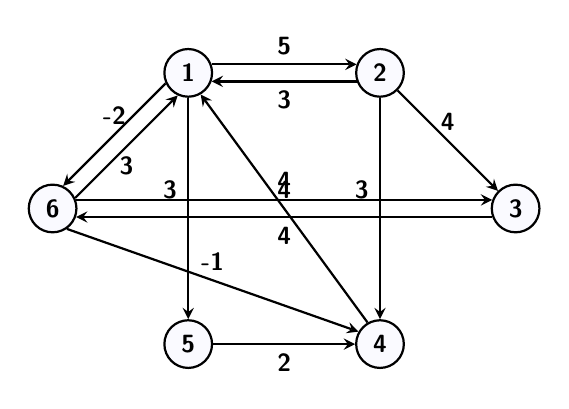
\begin{tikzpicture}[->,>=stealth,auto,node distance=7em, thick,main node/.style={circle,fill=blue!2,draw,font=\sffamily\small}] font=\sffamily\small\bfseries \node[main node] (1) {1}; 
\node[main node] (2) [right of=1] {2}; 
\node[main node] (3) [below right of=2] {3}; 
\node[main node] (4) [below left of=3] {4}; 
\node[main node] (5) [left of=4] {5}; 
\node[main node] (6) [below left of=1] {6};
\draw (1.20) -- (2.160) node[midway, above] {5};
\draw (2.200) -- (1.-20) node[midway, below] {3};
\draw (2.-45) -- (3.135) node[midway, above] {4};
\draw (5.0) -- (4.180) node[midway, below] {2};
\draw (1.-155) -- (6.65) node[midway, above] {-2};
\draw (6.25) -- (1.-115) node[midway, below] {3};
\draw (6.20) -- (3.160) node[midway, above] {4};
\draw (3.200) -- (6.-20) node[midway, below] {4};
\draw (1.-90) -- (5.90) node[midway,above] {3~~~~~};
\draw (2.-90) -- (4.90) node[midway, above] {3~~~~~};
%\draw (4.120) -- (1.-55) node[pos=.2,above] {4x}
\draw (4.120) -- (1.-60) node[midway, above] {4};
\draw (6.-55) -- (4.150) node[midway, above] {-1};
\end{tikzpicture}

\begin{tikzpicture}[->,>=stealth',shorten >=1pt,auto,node distance=3cm,
thick,main node/.style={circle,fill=blue!20,draw,font=\sffamily\Large\bfseries}]
\node[main node] (1) {1};
\node[main node] (8) [ left of=1] {8};
\node[main node] (11) [ below of=1] {11};
\node[main node] (12) [ left of=8] {12};
\node[main node] (13) [ below of=12] {13};

\node[main node] (7) [ left of=13] {7};
\node[main node] (14) [ below left of=11] {14}; 
\node[main node] (10) [ below left of=14] {10};
\node[main node] (5) [below of=10]{5};
\node[main node] (9) [ right of=11] {9}; 
\node[main node] (2)  [below right of=14] {2};
\node[main node] (3) [ right of=2] {3};
\node[main node] (4) [below left of=2] {4};

\node[main node] (15) [ below right of=2] {15};
\node[main node] (16) [right of=3] {16};
\node[main node] (6) [ below of=16] {6};


\path[every node/.style={font=\sffamily\small}]
(1) edge node [left] {} (11)
(2) edge node [right] {} (11)
(3) edge node [right] {} (6)
edge node [right] {} (11)
edge node [right] {} (16)
(4) edge node [left] {} (2)
edge node [left] {} (10)
edge node [left] {} (11)
edge  [bend right] node{} (13)
edge node [bend right]{} (15)
(6)  edge[bend left] node [left] {} (5)
edge node [left] {} (15)
(8)  edge node [left] {} (11)
edge node [left] {} (2)
(9)  edge node [left] {} (11)
(10)edge node[left]{}  (2)
edge[bend left] node [left] {} (11)
(13) edge node [left] {} (11)
edge node [left] {} (12)
(14)  edge node [left] {} (2)
edge node [left] {} (4)
edge node [left] {} (8)
edge node [left] {} (10)
edge node [left] {} (11)
edge node [left] {} (13);
\end{tikzpicture}

\begin{tikzpicture}[>=latex,text height=1.5ex,text depth=0.25ex]
\matrix[row sep=0.5cm,column sep=0.5cm] {
	% First line: Control input
	&
	\node (y_0) [measurement] {$\mathbf{y}_{0}$}; &
	\node (y_1) [measurement] {$\mathbf{y}_{1}$}; &
	\node (y_2) [measurement] {$\mathbf{y}_{2}$}; &
	\node (y_3) [measurement] {$\mathbf{y}_{3}$}; &
	\\
	% Second line: System noise & input matrix
	\node ({S_{3}}') [input] {$\mathbf{S_{3}}'$}; &
	\node ({A_{0}}') [matrx] {$\mathbf{A_{0}}'$}; &
	\node ({A_{1}}') [matrx] {$\mathbf{A_{1}}'$}; &
	\node ({A_{2}}') [matrx] {$\mathbf{A_{2}}'$}; &
	\node ({A_{3}}') [matrx] {$\mathbf{A_{3}}'$}; &
	\node ({S_{0}}') [input] {$\mathbf{S_{0}}'$}; &
	\\
	\node ({S_{0}}) [input] {$\mathbf{S_{0}}$}; &
	\node ({A_{0}}) [matrx] {$\mathbf{A_{0}}$}; &
	\node ({A_{1}}) [matrx] {$\mathbf{A_{1}}$}; &
	\node ({A_{2}}) [matrx] {$\mathbf{A_{2}}$}; &
	\node ({A_{3}}) [matrx] {$\mathbf{A_{3}}$}; &
	\node ({S_{3}}) [input] {$\mathbf{S_{3}}$}; &
	\\
	% Fifth line: 输入
	&
	\node (x_0) [state]{$\mathbf{x}_{0}$}; &
	
	\node (x_1) [state2]{$\mathbf{x}_{1}$}; &
	
	\node (x_2)   [state3]{$\mathbf{x}_{2}$}; &
	
	\node (x_3) [state4]{$\mathbf{x}_{3}$}; &
	
	\\
};

% The diagram elements are now connected through arrows:
\path[->]
({S_{0}}') edge[thick] ({A_{3}}')
({A_{3}}') edge[thick] ({A_{2}}')
({A_{2}}') edge[thick] ({A_{1}}')
({A_{1}}') edge[thick] ({A_{0}}')
({A_{0}}') edge[thick] ({S_{3}}')

({S_{0}}) edge[thick] ({A_{0}})
({A_{0}}) edge[thick] ({A_{1}})
({A_{1}}) edge[thick] ({A_{2}})
({A_{2}}) edge[thick] ({A_{3}})
({A_{3}}) edge[thick] ({S_{3}})

(x_0) edge ({A_{0}})
(x_1) edge ({A_{1}})
(x_2) edge ({A_{2}})
(x_3) edge ({A_{3}})
({A_{0}}') edge (y_0)
({A_{1}}') edge (y_1)
({A_{2}}') edge (y_2)
({A_{3}}') edge (y_3)

(x_0) edge[->,bend right=37,green]	({A_{0}}')
(x_1) edge[->,bend right=37,green]	({A_{1}}')
(x_2) edge[->,bend right=37,green]	({A_{2}}')
(x_3) edge[->,bend right=37,green]	({A_{3}}')
({A_{3}}) edge[->,bend right=37,green]	(y_3)
({A_{2}}) edge[->,bend right=37,green]	(y_2)
({A_{1}}) edge[->,bend right=37,green]	(y_1)
({A_{0}}) edge[->,bend right=37,green]	(y_0)
;
\end{tikzpicture}

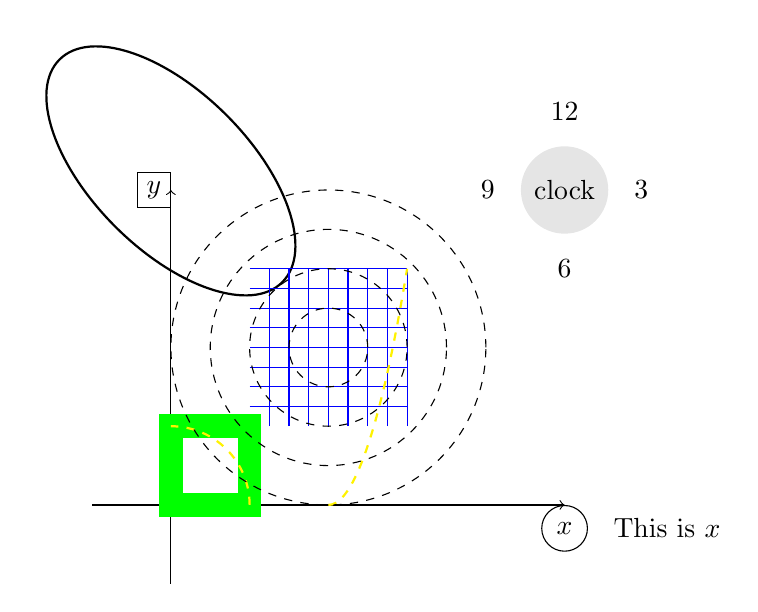
\begin{tikzpicture}[label distance = 2mm]

\draw[->] (-1,0) -- (5,0) node[below,circle,draw,label distance = 1cm,label=right:This is $x$] {$x$};
\draw[->] (0,-1) -- (0,4) node[left,rectangle,draw] {$y$};
\draw[color = green,line width = 3mm] (0,0) -- plot coordinates {(1,0)  (1,1)  (0,1)} -- cycle;
\draw[color = black,thick,rotate = 45] (3,3) circle (1cm and 2cm);
\draw[step=0.25cm,color = blue] (1,1) grid (3,3);
\tikzstyle{my style}=[yellow,dashed,thick];
\draw[style = my style] (2,0) parabola (3,3);
\draw[style = my style] (1,0) arc (0:90:1cm);

\begin{scope}[dashed]
\draw (2,2) circle (2cm);
\draw (2,2) circle (1.5cm);
\draw (2,2) circle (1cm);
\draw (2,2) circle (0.5cm);
\end{scope}
\draw (5,4) node [circle,fill=gray!20,label = right:3,label=above:12,label=below:6,label = left:9]{clock};
\draw [thick,dashed,domain=0:2] plot[id = x] function {x*x};
\draw [thick,domain=0:1.5] plot [id = x] function {2*x*x};
\end{tikzpicture}
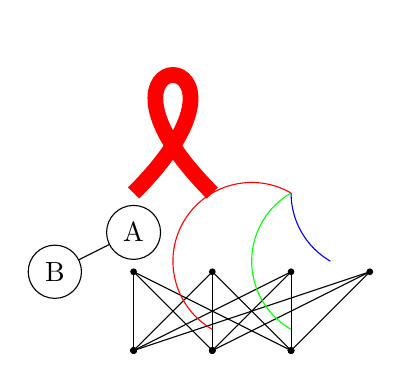
\begin{tikzpicture}
\draw[line width=0.2cm,red] (1,1) .. controls (3,3)
and (0,3) .. (2,1);
%\draw (1,0.5) node[draw,shape=circle,anchor=south west]{A} -- (0,0) node[draw,shape=circle,anchor=north east]{B};
\path (1,0.5) node[draw,shape=circle](v0){A};
\path (0,0) node[draw,shape=circle](v1){B};
\draw (v0) -- (v1);

\foreach \i in {1,...,4}
{
	\filldraw[black] (\i,0) circle (1pt);
	\foreach \j in {1,...,3}
	{
		\filldraw[black] (\j,-1) circle (1pt);
		\draw (\i,0) -- (\j,-1);
	}
}

%  \foreach \i/\j in {60/red,120/green,180/blue}
%  {
%    \draw[\j] (1,1) arc (\i:240:1cm);
%  }
\draw[red] (3,1) arc (60:240:1cm);
\draw[green] (3,1) arc (120:240:1cm);
\draw[blue] (3,1) arc (180:240:1cm);

\end{tikzpicture}

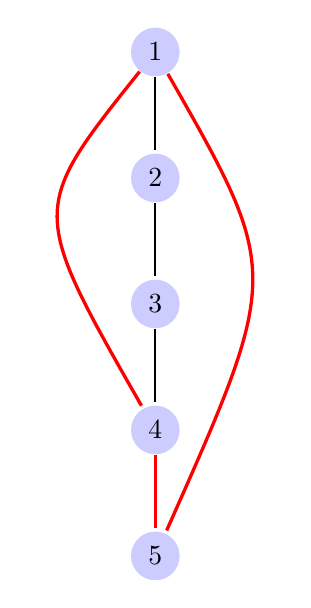
\begin{tikzpicture}[> = stealth, % arrow head style
shorten > = 1pt, % don't touch arrow head to node
auto,
node distance = 3cm, % distance between nodes
semithick % line style
,scale=.8,auto=left,every node/.style={circle,fill=blue!20}]
\node (n1) at (0,0)		{1};
\node (n2) at (0,-2)  	{2};
\node (n3) at (0,-4) 	{3};
\node (n4) at (0,-6) 	{4};
\node (n5) at (0,-8) 	{5};
\draw (n1)--(n2);
\draw (n2)--(n3);
\draw (n3)--(n4);
\draw [red,very thick](n4)--(n5);
\draw [red,very thick] (n1) .. controls (-2,-2.5)  ..(n4);
\draw [red,very thick](n1) .. controls (2,-3.5) 	..(n5);
\end{tikzpicture}

过程介绍:
\begin{enumerate}
	\item 包含tikz宏包,并且载入要使用的库。在本例中就是
	\lstinline{tikz}与
	\lstinline{positioning,arrows.meta}两条命令;
	\item 先定义好需要的样式(style)。本例中先定义了要用到的方框与箭头的样式。当然,这是因为有现成的图形参照,如果没有也可后面再定义。先定义好需要的样式(style)。一般我会把style单独放在一个文件中由主文件来调用;
	\item 绘制方框后连线。
\end{enumerate}
说明:
\begin{enumerate}
	\item 绘制方框的语句格式一般是
	\begin{lstlisting}
	\node[样式](名称){标题};
	\end{lstlisting}
	注意结尾的分号,绘制线条的语句最后先要加分号。名称是调用时使用,可以用汉字,标题是显示出来的文字,二者不一样;
	\item 样式的内容挺多的,方框中一般会用到形状(shape)、边框颜色(draw)、填充色(fill)、宽度(text width)、最小高度(minimum height)。颜色方面可以参考xcolor宏包的说明文档。长度单位有好几个,我一般常用的是pt与cm,1pt=0.351mm;
	\item 位置的表示也包含在样式定义中,一般形式是:方位 = 尺寸 of 参考对象。方位包括left、right、below、above、below left、below right、above left、above right 8种,要注意below left这样的顺序不能颠倒;
	\item 这里我们绘制箭头的库选用的是arrows.meta(24种箭头),这个库比arrows(14种)要丰富些。箭头的形状有很多种,详情请参考\href{https://stuff.mit.edu/afs/athena/contrib/tex-contrib/beamer/pgf-1.01/doc/generic/pgf/version-for-tex4ht/en/pgfmanualse24.html}{arrows.meta的24种箭头},本例中箭头样式选的是Latex样式,其后的length = 4mm, width = 1.5mm代表箭头的长宽,可以通过这两个参数调整箭头的锋锐程度。大家可以根据需要设置;
	\item 在线条上加文字的方法是通过加入node来实现,注意node在连线(即–)中的位置,如果放在–左边就表示文字是在线段的左边,反之在右边。实际上我们可以通过xshift、yshift两个参数来随意调整位置;
	\item 语句
	\begin{lstlisting}
	\draw[arrow1](0, 50pt)node[right, yshift = -15pt]{输入源程序} -- (词法);
	\end{lstlisting}
	其中的(0, 50pt)是指在绝对坐标0, 50pt处开始绘制,图形坐标的原点(0, 0)就是代码中第一个方框的中心处。如果我们在(0, 50pt)前加两个加号,例如++(0, 50pt),那就变成了相对坐标,是相对于上一个节点。例如语句:
	\begin{lstlisting}
	\draw[arrow1](生成) -- node[right, yshift = 5pt, xshift = 5pt]{目标代码}++(0, -50pt);
	\end{lstlisting}
	++(0, -50pt)的意思就是相对于“生成”这个节点向下移动50pt的坐标。当我们不清楚绝对坐标时就用相对坐标来绘制,挺方便的。
\end{enumerate}
% 定义方框样式
\tikzset{
	rect1/.style = {
		shape = rectangle,
		draw = green,
		text width = 3cm,
		align = center,
		minimum height = 1cm,
	}
}
% 定义箭头样式
\tikzset{
	arrow1/.style = {
		draw = purple, thick, -{Latex[length = 4mm, width = 1.5mm]},
	}
}
% 双箭头
\tikzset{
	arrow2/.style = {
		draw = purple, thick, {Latex[length = 4mm, width = 1.5mm]}-{Latex[length = 4mm, width = 1.5mm]},
	}
}
\begin{center}
	\begin{tikzpicture}
	% 绘制中间方框
	\node[rect1, fill = green!60!white](词法){词法分析};
	\node[rect1, fill = green!40!white, below = of 词法](语法){语法分析};
	\node[rect1, fill = green!20!white, below = of 语法, text width = 5cm](语义中间){语义分析、中间表示生成};
	\node[rect1, fill = green!60!black, below = of 语义中间](优化){\color{white}代码优化};
	\node[rect1, fill = green!30!black, below = of 优化](生成){\color{white}代码生成};
	% 绘制两侧方框
	\node[rectangle, fill = red!20!white, draw = red, text width = 0.7cm, minimum height = 4cm, align = center, left = 2cm of 语义中间](符号){符号表管理};
	\node[rectangle, fill = blue!20!white, draw = blue, text width = 0.7cm, minimum height = 4cm, align = center, right = 2cm of 语义中间](出错处理){出错处理};
	% 绘制中间连线
	\draw[arrow1](0, 50pt)node[right, yshift = -15pt]{输入源程序} -- (词法);
	\draw[arrow1](词法) -- node[right]{单词流}(语法);
	\draw[arrow1](语法) -- node[right]{文法}(语义中间);
	\draw[arrow1](语义中间) -- node[right]{中间表示}(优化);
	\draw[arrow1](优化) -- node[right]{优化后中间表示}(生成);
	\draw[arrow1](生成) -- node[right, yshift = 5pt, xshift = 5pt]{目标代码}++(0, -50pt);
	% 绘制两侧连线
	\draw[arrow2](符号) -- (词法.west);
	\draw[arrow2](符号) -- (语法.west);
	\draw[arrow2](符号) -- (语义中间);
	\draw[arrow2](符号) -- (优化.west);
	\draw[arrow2](符号) -- (生成.west);
	\draw[arrow2](出错处理) -- (词法.east);
	\draw[arrow2](出错处理) -- (语法.east);
	\draw[arrow2](出错处理) -- (语义中间);
	\draw[arrow2](出错处理) -- (优化.east);
	\draw[arrow2](出错处理) -- (生成.east);
	% 绘制虚线框
	\draw[thick, dashed, draw = purple](-125pt, 27pt)node[below right]{编译器前端} -- (125pt, 27pt) -- (125pt, -250pt) -- (-125pt, -250pt)node[above right]{编译器后端} -- (-125pt, 27pt);
	\draw[thick, dashed, draw = purple](-125pt, -135pt) -- (125pt, -135pt);
	\end{tikzpicture}
	\\ 编译器结构图
\end{center}

\begin{tikzpicture}[domain=-4:3.5,line width=2pt]
\clip (-5,-5) rectangle (6,6);%只在这个区域内画图
%绘制网格
\draw[ thin,color=gray] (-4,-2) grid (4,4);
%绘制y=sin(x)
\draw[color=blue,name path=c1] plot (\x,{sin(\x r)})
node[right] {$f(x) = \sin x$};
%绘制y= 0.1 * e^ x
\draw[color=black,name path=c2] plot (\x,{0.1*exp(\x)})
node[right] {$f(x) = 0.1 *\mathrm{e}^ x$}; 
%求交点, i-\s是每个交点的名称.i是前缀  \t表示总的交点数   
\fill [name intersections ={of ={ c1 and c2},name=i,total=\t}]
\foreach \s in {1,...,\t}{(i-\s) circle(3pt) node[above]{\s}};
\end{tikzpicture}

下面两个函数表达式:
\[
\sgn\left(x\right)=\left\{\begin{array}{l}
1,x\geq 0\\
0,x<0\\
\end{array}\right. 
\]
\[
\textrm{sigmoid}\left(x\right)=\frac{1}{1+\textrm{e}^{-x}}
\]
\begin{center}
\begin{tikzpicture}
\draw[->](-1.2,0)--(1.2,0)node[left,below,font=\tiny]{$x$};
\draw[->](0,-0.2)--(0,1.2)node[right,font=\tiny]{$y$};
\foreach \x in {-1,0,1}{\draw(\x,0)--(\x,0.05)node[below,outer sep=2pt,font=\tiny]at(\x,0){\x};}
\foreach \y in {1}{\draw(0,\y)--(0.05,\y)node[left,outer sep=2pt,font=\tiny]at(0,\y){\y};}
\draw[color=red, thick,smooth,domain=0:1]plot(\x,1);
\draw[color=red, thick,smooth,domain=-1:-0.02]plot(\x,0);
\draw[color=red,smooth]circle(0.02);
\end{tikzpicture}
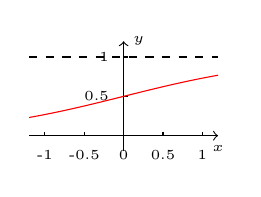
\begin{tikzpicture}
\draw[->](-1.2,0)--(1.2,0)node[left,below,font=\tiny]{$x$};
\draw[->](0,-0.2)--(0,1.2)node[right,font=\tiny]{$y$};
\draw[dashed](-1.2,1)--(1.2,1);
\foreach \x in {-1,-0.5,0,0.5,1}{\draw(\x,0)--(\x,0.05)node[below,outer sep=2pt,font=\tiny]at(\x,0){\x};}
\foreach \y in {0.5,1}{\draw(0,\y)--(0.05,\y)node[left,outer sep=2pt,font=\tiny]at(0,\y){\y};}
\draw[color=red ,domain=-1.2:1.2]plot(\x,{1/(1+(e^(-1*(\x))))});
\end{tikzpicture}
\end{center}